\section{Probes}
\label{sec:method}

\subsection{Normalisation}
Every probe reads a triangle mesh after a deterministic normalisation.
The bounding box is centred at the origin and scaled so that its diagonal equals 1.
Vertices are then welded by rounding coordinates to \(10^{-6}\) and replacing each welded group by its mean.
All lengths reported below are therefore in units of the bounding-box diagonal, and the probes have no learned parameters.
Area-weighted samples use a fixed random seed, so a given file and library build produce the same scalars.
Configuration constants are collected in Appendix~\ref{app:probes}.
% src: geomcheck/probes.py

When a mesh has more than 10{,}000 faces we optionally decimate it, before probing, to 10{,}000 faces by quadric edge collapse with topology, boundary and normal preservation and planar quadrics enabled \citep{garland1997qem,cignoni2008meshlab}.
3D-DefectBench meshes already lie at or below about 10.7k faces (median 8{,}119), which is the regime in which the classifier was trained, so the expert-set evaluation does not decimate.
MATE-3D and the GSO injection study do.
A faster decimator was rejected before any scoring because it opened holes; that deviation is recorded in Appendix~\ref{app:prereg}.
% src: results/RESULTS_milestone1.md; results/runtime_summary.csv; geomcheck/probes.py; analysis/PREREGISTRATION_M2.md

\subsection{Feature families}
We compute eight feature families (size, boundary/manifold, topology, triangle quality, roughness, self-intersection, hidden surface and thin wall), described in six groups below.
Unless noted, fractions are over faces, edges or samples as stated.

\paragraph{Size and boundary.}
Face count; fraction of duplicate faces; fraction and total length of boundary edges; number of boundary loops; fraction of two-manifold edges whose two directed half-edges fail to cancel (winding); fraction of non-manifold edges.
A mesh is recorded as watertight when it has no boundary and no non-manifold edge.

\paragraph{Topology.}
Face-adjacency components, the area fraction of the largest component, the number and area fraction of components smaller than 1\% of the surface, and the number of remaining components.
The genus proxy is
\begin{equation}
g = \max\bigl(0,\, 2C - \chi\bigr) / 2,
\label{eq:genus}
\end{equation}
where \(C\) is the number of components and \(\chi = V - E + F\), with \(V\) the number of vertices referenced by a face.
The classifier receives \(\log(1+g)\).

\paragraph{Triangle quality.}
For a triangle of area \(A\) and edge lengths \(a,b,c\),
\(q = 4\sqrt{3}\, A / (a^2+b^2+c^2)\), which equals 1 for an equilateral triangle and 0 for a degenerate one.
We store the median and the 5th percentile of \(q\), the fraction of faces and of area with \(q < 0.1\) (slivers), and the coefficient of variation of edge length.

\paragraph{Roughness.}
On each interior manifold edge we take the angle between the two incident face normals.
We store the length-weighted mean angle in degrees and the length fraction above \(30^\circ\), \(60^\circ\) and \(90^\circ\), plus the mean and 95th percentile of absolute angle defect on interior manifold vertices.

\paragraph{Self-intersection.}
PyMeshLab marks faces that intersect another face of the same mesh \citep{cignoni2008meshlab}.
We store the fraction of faces and of area that are marked.

\paragraph{Hidden surface and thin walls.}
We draw 20{,}000 area-weighted points on the surface.
A point is hidden when a ray from it fails to escape in every one of 64 Fibonacci directions (Embree) \citep{wald2014embree}.
Thickness at a point is the length of the shorter ray along the outward or inward normal that exits through a face whose normal agrees with the ray.
We store the fraction of samples at which thickness is defined, the median thickness, and the fraction of samples thinner than \(0.005\) and \(0.010\) diagonals.
% src: geomcheck/probes.py

Features with zero variance on the training split were dropped.
The classifier uses the remaining 30 features.
Figure~\ref{fig:pipeline} shows the path from a file to those features and to the frozen scores.

\begin{figure}[t]
  \centering
  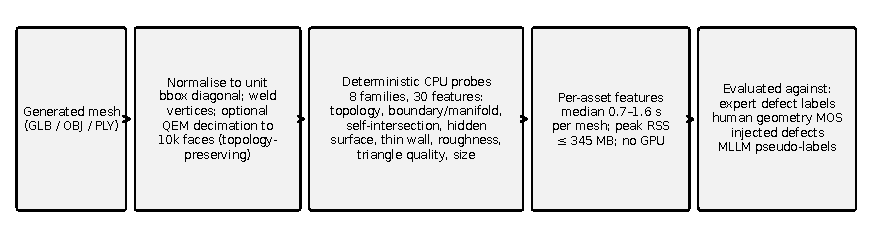
\includegraphics[width=\linewidth]{figures/fig1a_pipeline.pdf}
  \caption{Probe pipeline. A mesh is normalised to a unit bounding-box diagonal, welded, and, outside 3D-DefectBench, decimated to 10{,}000 faces. Deterministic features are then passed to a logistic regression whose weights and thresholds were frozen on the silver holdout.}
  \label{fig:pipeline}
\end{figure}

\subsection{Frozen classifier and controls}
The primary predictor, GeomProbe-LR, is one L2 logistic regression per defect.
Features are transformed by \(\log(1+x)\) (genus as above) and standardised with the mean and variance of the training split.
The regression uses \(C = 1\), balanced class weights and at most 5{,}000 iterations.
The decision threshold maximises Matthews correlation coefficient (MCC) on the five-fold stratified out-of-fold probabilities of the training split (shuffle, seed 0).
The model is then refit on the whole training split.
Nothing---features, \(C\), or thresholds---was chosen on the expert set.
% src: analysis/PREREGISTRATION.md

Two controls use the same threshold rule.
FaceCount-LR sees only \(\log(1+n_{\text{faces}})\).
Generator-only sees only the generator identity.
For 3D-DefectBench that identity is the benchmark's model A or model B.
We also report the within-generator AUROC of GeomProbe-LR so that a between-generator difference is not mistaken for a geometric effect.

VLM comparisons use the binary votes released with 3D-DefectBench (configuration c004, successfully parsed rows only) \citep{zhao2026defectbench}.
For a binary vote, AUROC equals balanced accuracy; we label it as such.
Probe AUROC uses the predicted probability.
MCC and F1 are computed for every predictor.
Our macro-MCC values for the 12 VLMs reproduce those reported by the benchmark authors to three decimal places; the match was checked before the expert-set plan was written, as a label-handling test, and it is not a result about geometry.
% src: analysis/PREREGISTRATION.md; results/RESULTS_milestone1.md

\subsection{Injection operators}
On each cleaned GSO mesh we apply seven operators at three severities (S1 \(<\) S2 \(<\) S3), using a per-object seed.
Holes delete three surface patches whose total area is 0.2\%, 1\% or 4\% of the mesh.
Floaters add 1, 3 or 10 icospheres of radius 0.01, centred 0.05 off the surface along the normal.
An interpenetrating part is an ellipsoid of major radius 0.05, 0.10 or 0.20, concatenated without a Boolean union.
A thin fin is a \(0.2 \times 0.2\) plate of thickness 0.008, 0.004 or 0.002, half-embedded at a surface point.
Noise displaces vertices along their normals by a Gaussian of standard deviation 0.001, 0.003 or 0.01.
A crossing sheet duplicates a patch of area 0.5\%, 2\% or 5\% and rotates the copy by \(30^\circ\).
A hidden shell places an icosphere, of radius 0.25, 0.50 or 0.90 times the distance from an interior point to the surface, at the point farthest from the surface among 20{,}000 uniformly sampled interior candidates.
Objects with no interior point would have been skipped and counted; none were.
% src: scripts/gso_inject.py; analysis/PREREGISTRATION_M2.md; results/RESULTS_milestone2.md

Each operator has a pre-registered target check.
Holes map to boundary-edge fraction, and floaters to the small-component count.
Interpenetration maps to self-intersection and also to hidden surface.
Fins map to the thin-wall fraction at 0.005, and noise to the length-weighted dihedral mean.
Crossing sheets map to self-intersection, and internal shells to hidden surface.
S1 fins are thicker than 0.005 by design.
The 0.010 thin-wall check is the one expected to see them.
% src: analysis/PREREGISTRATION_M2.md; results/RESULTS_milestone2.md
